\addtocontents{toc}{\setcounter{tocdepth}{3}}

\chapter{Initialisation du projet}

\section*{Introduction}
Dans ce chapitre, la première étape de Scrum qui est l'initialisation du projet sera traitée. C'est en fait à propos de
la phase de définition de l'architecture du produit à produire et la préparation de l'environnement de développement. Cette phase ne se termine pas par une livraison.

\section{Environnement de développement}
Dans cette section, nous allons présenter les outils et les technologies utilisés pour la conception et la réalisation de notre application.
\subsection{Environnement matériel}
Pour élaborer ce projet, un micro-ordinateur portable DELL E5540 fourni par la société a été utilisé. Il est exploité sous le système d’exploitation Windows 7 et il possède les caractéristiques suivantes :
 \begin{itemize}
    \item Processeur Intel Core i5-4210 U, 2.40 GHz;
    \item Mémoire vive «RAM» d’une capacité de 8 GO;
    \item Disque dur d’une capacité de 1 TO;
    \item Ecran de 15,6 pouces.
    \end{itemize}
\subsection{Environnement logiciel}
\textbf{Outil de modélisation UML : PowerAMC }\\
L’outil «PowerAMC» offre plusieurs méthodes de modélisation, accessibles aux informaticiens de tout niveau, parmi elles : Merise, UML, Data Warehouse, et processus métiers \cite{PowerAmc}.\\
   Cet outil est retenu pour la représentation des schémas des différents diagrammes (d’utilisation, de classes et de séquences).

\textbf{Environnement de développement intégré (IDE) : Intellij IDEA}\\
IntelliJ IDEA est un environnement de développement intégré (IDE) largement destiné à des langages comme Java, Scala, Angular... \cite{IDEA}.
\\Nous avons utilisé cet environnement pour le développement de notre application avec Angular et Node.js.

\textbf{Postman}\\
c’est un outil fourni par Google permet d’appeler et tester une API Web.
\newpage
\textbf{Node.js}\\
Node. js est une plate-forme pour la construction des applications serveurs rapides et évolutives en JavaScript \cite{NodeJs}.\\
Notre choix a été basé sur Node.js vu que notre application est une application web dynamique qui demande de la performance et de la portabilité.

\textbf{HTML 5 / CSS 3}\\
HTML est considéré comme un langage de balisage qui a pour but d'organiser et de structurer des pages web. CSS est le complémentaire de HTML, permet de définir des styles de ces pages \cite{HTMLCSS}.\\
Les versions 3 et 5 ont été choisies et utilisées respectivement pour CSS et HTML dans le but de créer des interfaces graphiques pour notre application.

\textbf{Javascript}\\
JavaScript est le langage de programmation du HTML et du Web. Il est utilisé dans les pages web interactives \cite{JavaScript}. 

\textbf{Bootstrap}\\
Bootstrap est le framework HTML, CSS et JavaScript le plus populaire pour le développement des sites web réactifs et mobiles \cite{BootStrap}.\\
La version 4 de cette technologie a été choisie et qui a été utilisée pour améliorer et fournir une interface conviviale.

\textbf{Angular 4}\\
Angular 4 est un framework javascript qui facilite la création d'applications sur le web. Il combine les modèles déclaratifs, l'injection de dépendance et les meilleures pratiques intégrées pour résoudre les problèmes de développement \cite{Angular}.

\textbf{MongoDb}\\
MongoDB stocke des données dans des documents flexibles de type JSON, ce qui signifie que les champs peuvent varier d'un document à un autre et que la structure des données peut être modifiée au fil du temps \cite{MongoDb}.\\ La version 3 de Mongodb a été choisie dans l'objectif de gérer de grandes quantités de données.

\textbf{Python}\\
Python est un langage de programmation interprété, interactif, orienté objet et de haut niveau.\\ Nous avons réalisé notre modèle de prédiction avec Python et précisément avec Tensorflow \cite{Python}.
\newpage
\textbf{TensorFlow}\\
TensorFlow est un framework de programmation pour le calcul numérique qui a été rendu open source par Google en Novembre 2015. Depuis sa sortie, TensorFlow n’a cessé de gagner en popularité, pour devenir très rapidement l’un des frameworks les plus utilisés pour le Machine learning et Deep learning, comme le montrent les dernières comparaisons suivantes, faites par François Chollet (auteur de la librairie Keras).

\begin{figure}[htpb]
    \centering
    \fcolorbox{brown}{white}{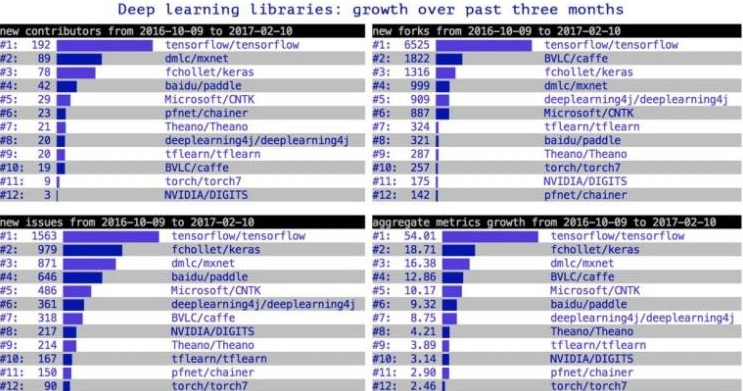
\includegraphics[width=1\linewidth]{img/deep_learning_tensorflow.png}}
    \caption{Évolution des bibliothèques Deep Learning}
    \label{fig:tensorflowDeepLearning}
    \end{figure}

Parmi les avantages de Tensorflow : 
\begin{itemize}
    \item Compatibilité avec multi-plateformes (Linux, Mac OS, et même Android et iOS);
    
    \item Exposition des APIs en Python, C++, Java et Go;
    
      \item Temps de compilation très courts;
      
      \item Prise en charge des calculs sur CPU et GPU;
      
      \item Documentation extrêmement bien fournie avec de nombreux exemples et tutoriels.
   
    \end{itemize}
Alors qu'il a été développé pour optimiser les calculs numériques complexes, Tensorflow est aujourd’hui particulièrement plus utilisé pour le deep learning (réseaux de neurones) \cite{Tensorflow}.
\\
\textbf{Flask :}\\
Nous avons utilisé Flask pour exposer les différentes phases (import des données, préparation des données, création du modèle de prédiction….) sous format des services web (API REST) dans le but d’interagir avec Node.js via un format JSON.

\section{Architecture de l'application}
Dans cette section, nous allons présenter l'architecture physique et logicielle de notre application.
\subsection{Architecture physique de l'application}
Pour la réalisation de nos systèmes, nous avons adopté l'architecture 3-tiers. Ce modèle d'architecture est décomposé en 3 parties logiques distinctes, chacune ayant un rôle bien défini :
\begin{itemize}
    \item Le client qui correspond dans notre cas à un navigateur dans l’ordinateur ou le téléphone d’un utilisateur. Son rôle est d'afficher les données et de permettre à l'utilisateur final d'interagir avec elles;
    
    \item Le serveur web reçoit une demande du client, la traite et fait appel au serveur de base de données, pour servir le client;
    
      \item Le serveur de données, fournissant au serveur web les données dont il a besoin. 
   
   
    \end{itemize}
La figure \ref{fig:architecture_physique} représente l'architecture physique de l'application.
    \begin{figure}[htpb]
    \centering
    \fcolorbox{brown}{white}{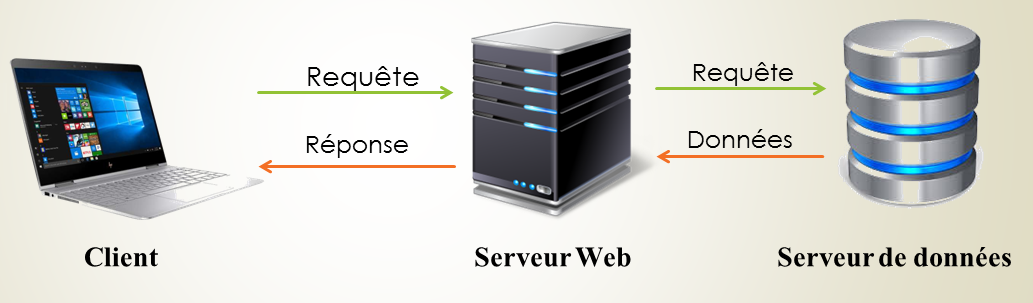
\includegraphics[width=1\linewidth]{img/architecture_physique_application_final.png}}
    \caption{Architecture physique de l'application}
    \label{fig:architecture_physique}
    \end{figure}
\subsection{Architecture logicielle de l'application}
La définition de l'architecture de l'application est une phase primordiale dans le processus de conception. Elle dépend d'un nombre de paramètres dont les besoins en matière de
la performance, les perspectives, l'évolutivité, la modularité et l'extensibilité.\\
La figure \ref{fig:architecture de projet} illustre une
représentation de l'architecture de notre application.
\newpage
    \begin{figure}[htpb]
    \centering
    \fcolorbox{brown}{white}{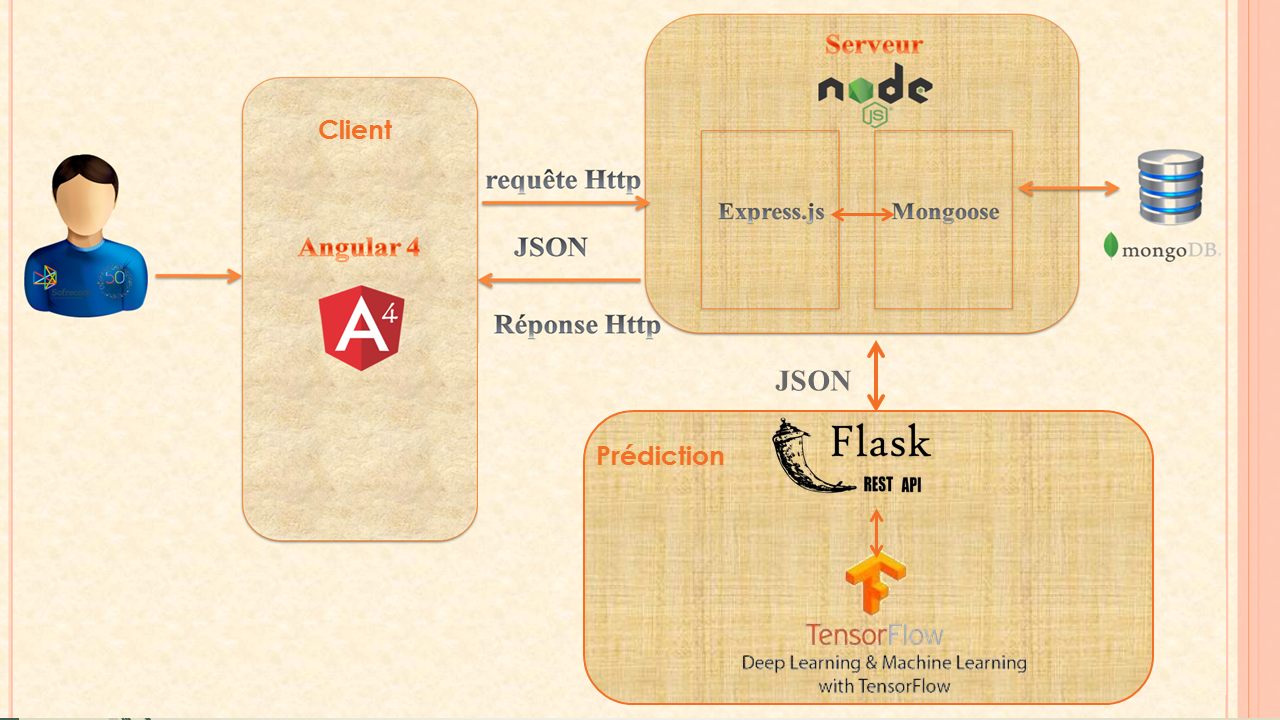
\includegraphics[width=1\linewidth]{img/architecture_de_sofrecom.png}}
    \caption{Architecture logicielle de l'application}
    \label{fig:architecture de projet}
    \end{figure}
   
Pour mieux comprendre cette architecture, nous allons procéder à l'explication des différentes parties :
 \begin{itemize}
    \item Au niveau du client, nous avons adopté le framework Angular version 4 qui nous permet de réaliser une application web monopage (Single Page Application). Cette dernière assure la fluidité de l'expérience utilisateur et évite le chargement d'une nouvelle page à chaque action demandée;
    
    \item Sur la partie serveur, nous avons opté pour le framework léger Express.js (basé sur node.js) pour recevoir et interpréter les requêtes entrantes du côté client et interagir avec la base de données Nosql MongoDB à travers le framework de node.js Mongoose.
    Mongoose est un Mappeur de document d'objet (Object Document Mapper ou ODM) qui permet de définir des objets avec un schéma fortement typé qui est mappé à un document MongoDB;
    
      \item  Les différentes phases de préparation des données, de construction du modèle de prédiction et d'évaluation du service de prédiction sont réalisées avec Tensorflow (basé sur python). Elles sont exposées au format des services web (API REST) pour interagir avec le serveur node.js à travers le framework Express.js. 
   
   
    \end{itemize}

\section{Diagramme de déploiement}
Ce diagramme décrit le déploiement de notre architecture logicielle.
En effet, il permet de décrire la disposition physique des ressources matérielles qui constituent notre système et de montrer la distribution des composants sur ces matériels. Le diagramme de déploiement modélise les ressources matérielles par des nœuds, et spécifie les liaisons entre eux \cite{DiagrammeDeploiement}.\\
La figure \ref{fig:Diagramme de déploiement} présente le diagramme de déploiement de notre application.
      \begin{figure}[htpb]
\centering
\fcolorbox{brown}{white}{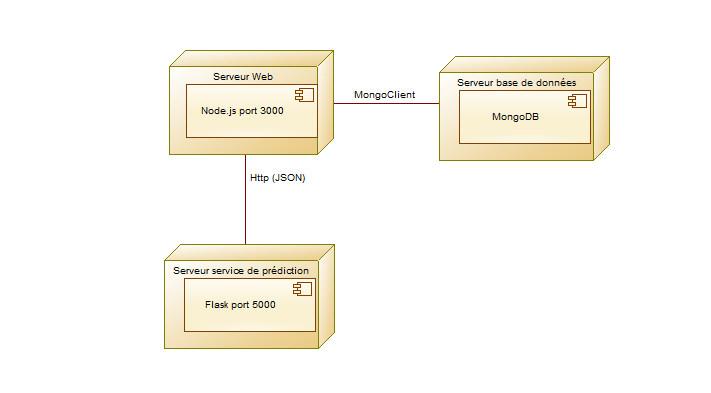
\includegraphics[width=1\linewidth]{img/deploiementDiagramme.png}}
\caption{Diagramme de déploiement}
\label{fig:Diagramme de déploiement}
\end{figure}

\section{Architecture des composants Angular}     
\begin{comment}Ce diagramme illustre l'architecture d'une application en termes de composants réutilisables.\\
\end{comment}
Nous allons nous intéresser à la partie front de notre application développée avec le framework Angular version 4.
En effet,  Angular 4 est orienté composant et chaque composant est défini comme étant un élément réutilisable \cite{diagComposant}.\\
La figure \ref{fig:Diagramme de composants} illustre l'architecture des composants de notre partie front où nous
distinguons, en rose les fichiers HTML, en orange les fichiers
TypeScript, en vert les fichiers
CSS et en bleu le paquetage ou composant qui englobe HTML, CSS et TypeScript.
Les flèches désignent une relation d’utilisation, par exemple Root Component utilise SideBar Component
qui utilise lui-même Utilisateur Component.
\newpage
      \begin{figure}[htpb]
\centering
\fcolorbox{brown}{white}{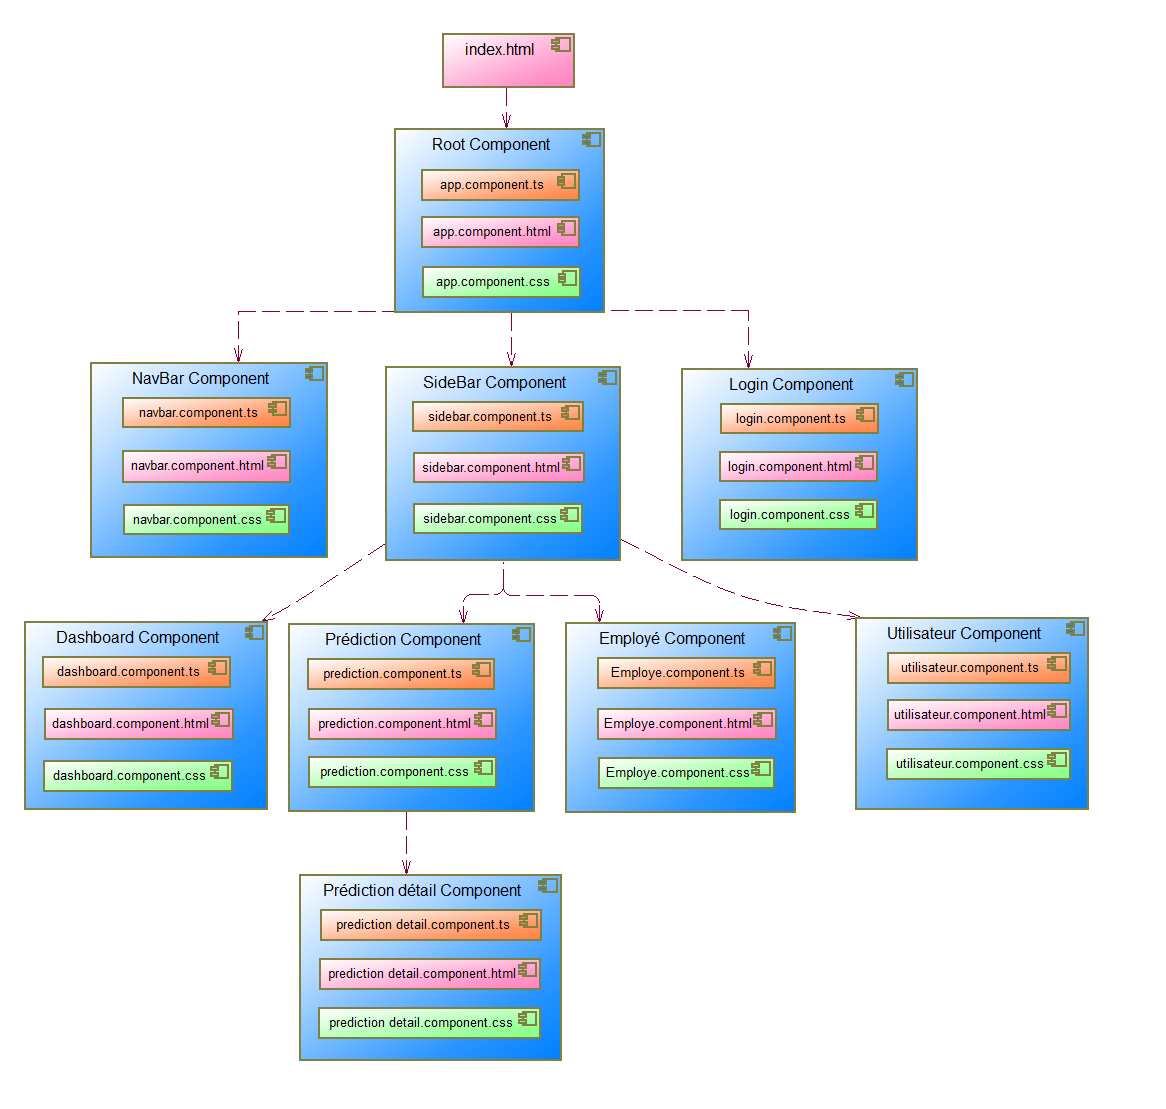
\includegraphics[width=1\linewidth]{img/DiagrammeComposant4_2_final.png}}
\caption{Architecture des composants Angular}
\label{fig:Diagramme de composants}
\end{figure}

Un composant fonctionne en associant la logique d'une classe TypeScript avec un template HTML et un style CSS.
Pour notre diagramme, le point d'entrée c'est le fichier index.html qui est notre unique page web comportant le Root Component. Cette page n’est
autre qu’un arbre de composants. Le Root component fait appel à d'autres composants qui peuvent aussi intégrer plusieurs composants.
\section*{Conclusion}
  À travers ce chapitre, nous avons présenté l'environnement de développement de notre application en justifiant nos choix technologiques. Le chapitre suivant sera consacré à la présentation de notre première release.
  
